\documentclass[a4paper,12pt]{article}
\usepackage[utf8]{inputenc}
\usepackage[T2A]{fontenc}
\usepackage[russian]{babel}
\usepackage{amsmath,amssymb,amsfonts}
\usepackage{graphicx}
\usepackage{array}
\usepackage{booktabs}
\usepackage{geometry}
\geometry{top=2cm,bottom=2cm,left=2.5cm,right=2.5cm}
\usepackage{indentfirst}

\DeclareMathOperator{\rank}{rank}

\title{Истинно случайные генераторы и скрытая передача ключей}
\author{Рустам Латыпов \\ 
Кафедра системного анализа и информационных технологий \\
Казанский федеральный университет, Казань, Россия \\
Roustam.Latypov@kpfu.ru \and
Евгений Столов \\
Кафедра системного анализа и информационных технологий \\
Казанский федеральный университет, Казань, Россия \\
ystolov@kpfu.ru}
\date{}

\begin{document}

\maketitle

\begin{abstract}
Большинство промышленных автоматических систем управляются удалённо, поэтому проблема защиты управляющей информации, передаваемой по открытому каналу, актуальна. Использование криптографических систем для безопасности предполагает возможность быстрого обмена системными ключами. В данной работе предлагается новое семейство истинно случайных генераторов ключей. Источником энтропии для таких случайных устройств является явление джиттера в электронных схемах. Генераторы строятся в виде каскадных схем на основе сумматоров. Мы даём архитектурное решение для синтеза генератора, основанного на динамике переходов такого устройства. Обсуждается процедура скрытой передачи ключей с использованием этих генераторов.
\end{abstract}

\textbf{Ключевые слова:} истинно случайные генераторы чисел, информационная безопасность, управление ключами.

\section{Введение}

Большинство промышленных устройств в настоящее время требуют доступа к Интернету. Компании не только продают систему один раз, но и сопровождают её в процессе использования, удалённо получая данные об устройстве, контролируя его состояние, проводя профилактические работы или даже полностью управляя производством [1--3]. Перенос информационных технологий в область автоматизации предоставит большие возможности.

С другой стороны, информация стала более важной, как и потребность в более сильной защите [4--6]. Безопасность на основе криптографических методов обычно используется во многих приложениях автоматизации из различных областей [7,8]. Если данные должны быть защищены от несанкционированного доступа, используется пароль или криптографическая система. Оба подхода должны поддерживаться генератором случайных значений [9,10]. В первом случае пароль генерируется генератором, во втором случае системные ключи должны быть случайными числами, которые генерируются специальным устройством или программой. Также такие генераторы могут быть частью системы, предназначенной для скрытой передачи данных. Для этих целей предпочтительны истинно случайные генераторы чисел.

В последнее время исследуется новое семейство таких генераторов. Они основаны на понятии джиттера комбинационной схемы с обратной связью [11,12]. Это явление возникает, если сигнал на входе комбинационной схемы зависит от выходов схемы.

Простейший вариант такого генератора представлен на рис.~1. Здесь инвертор используется как источник случайных чисел (джиттера). SR --- синхронный регистр, который сохраняет только тот выходной сигнал инвертора, который приходит с синхронизирующим импульсом. Регистр является обязательной частью любого генератора в нашем подходе, поэтому в дальнейшем мы не включаем SR в изображение при представлении структуры генератора.

\begin{figure}[h!]
\centering
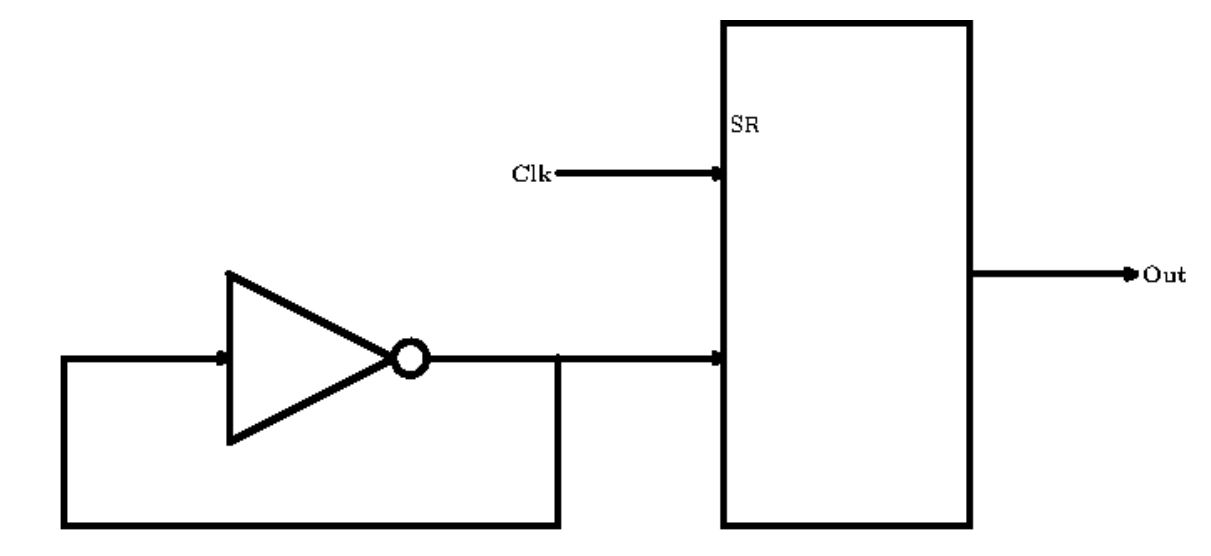
\includegraphics[width=0.55\textwidth]{Fig1.png}
\caption{Пример генератора, использующего явление джиттера.}
\label{fig:1}
\end{figure}

\section{Обзор литературы}

В этом разделе мы собираем все определения и результаты, относящиеся к рассматриваемому семейству генераторов. В нашем случае комбинационная схема, работающая в нестандартном режиме, состоит из сумматоров по модулю 2 над \(GF(2)\) [13]. Каждый вентиль имеет два входа и один выход. Некоторые входы вентилей могут быть свободными. Это означает, что на этот свободный вход подаётся постоянный сигнал. Для управления динамикой устройства мы используем эти сигналы на свободных входах. Существует обратная связь, которая может превратить схему либо в устройство с памятью, либо в генератор. Пример устройства представлен на рис.~2. Устройство состоит из 4 вентилей, два из которых имеют свободный вход. В наших предыдущих работах была разработана теория таких схем [14].

\begin{figure}[h!]
\centering
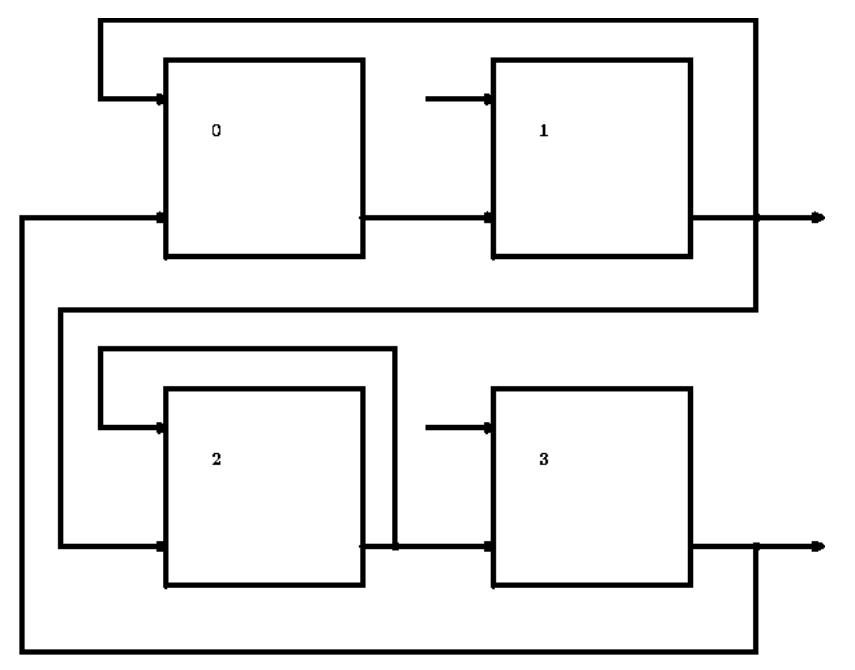
\includegraphics[width=0.6\textwidth]{Fig2.png}
\caption{Пример схемы, содержащей сумматоры по модулю 2 и обратную связь.}
\label{fig:2}
\end{figure}

\subsection{Матрица соединений}

Структура схемы может быть задана в терминах бинарной матрицы, то есть состоящей из единиц и нулей. Предположим, что в схеме \(N\) вентилей и \(M\) свободных входов. Матрица соединений \(\mathrm{Conn}\) имеет размер \(N \times (N + M)\). Пусть \(\mathrm{Conn}[i,j]\) --- элемент матрицы из \(i\)-й строки и \(j\)-го столбца, \(\mathrm{Conn}[I:J,P:Q]\) --- подматрица \(\mathrm{Conn}\), расположенная на пересечении строк с номерами \(I, I+1, \ldots, J-1\) и столбцов с номерами \(P, P+1, \ldots, Q-1\), \(\mathrm{Conn}[i,:]\) --- \(i\)-я строка матрицы. Аналогичные обозначения используются для доступа к компонентам векторов.

Все вентили пронумерованы целыми числами от \(0,1,\dots,N-1\). Свободные входы пронумерованы как \(0,1,\dots,M-1\). Элемент матрицы \(\mathrm{Conn}[i,j] = 1\), \(j < N\), тогда и только тогда, когда один из входов \(i\)-го вентиля соединён с выходом \(j\)-го вентиля. Элемент \(\mathrm{Conn}[i,j] = 1\), \(j \geq N\), тогда и только тогда, когда свободный вход с номером \(j - N\) соединён с одним из входов \(i\)-го вентиля. Это означает, что индекс этого свободного входа равен \(j - N\). Например, матрица соединений для схемы на рис.~\ref{fig:2} имеет вид

\[
\mathrm{Conn} =
\begin{pmatrix}
0 & 1 & 0 & 1 & 0 & 0 \\
1 & 0 & 0 & 0 & 1 & 0 \\
0 & 1 & 1 & 0 & 0 & 0 \\
0 & 0 & 1 & 0 & 0 & 1
\end{pmatrix}.
\]

Из определения следует, что в каждой строке матрицы \(\mathrm{Conn}\) ровно две единицы, а все остальные элементы --- нули. Каждый столбец матрицы может содержать произвольное число единиц. Очевидно, что по этой матрице можно восстановить схему с точностью до нумерации вентилей и входов.

\subsection{Динамика}

В [14] была предложена модель для описания динамики вышеупомянутого устройства. Она основана на уравнениях Эрланга для марковского процесса с непрерывным временем. Напомним основные факты, относящиеся к этой модели.

Пусть \(\alpha = \langle s_0, s_1, \ldots, s_{N-1} \rangle\) --- вектор, компоненты которого являются выходами всех вентилей в некоторый момент времени \(t\). Мы называем этот вектор состоянием устройства в момент времени \(t\). В дальнейшем будет использоваться вектор \(\gamma = \langle \alpha, \beta \rangle\), где \(\beta = \langle x_0, x_1, \ldots, x_{M-1} \rangle\) содержит все сигналы на свободных входах в этот момент. Мы обозначаем этот вектор как расширенное состояние схемы.

В соответствии с определением состояние устройства может измениться только в том случае, если один из вентилей изменит свой выход. Введём новую матричную операцию \(\Omega\):

\begin{equation}
\alpha' = \mathrm{Conn} \, \Omega_i \, \gamma^{\mathrm{T}}. \label{eq:1}
\end{equation}

Смысл этой операции таков: \(\alpha'[j] = \alpha[j]\) при \(j \neq i\) и \(\alpha'[i] = \mathrm{Conn}[i,*] \, \gamma^{\mathrm{T}}\) --- обычное матричное произведение [15,16]. С точки зрения вентилей, сумматор с номером \(i\) выполняет сложение сигналов на своих входах. Фактически возможно, что выход вентиля останется таким же, как и до операции, но мы рассматриваем эту ситуацию так, как если бы сумматор выполнил суммирование.

Применяя формулу \eqref{eq:1}, строят матрицу переходов \(T_{r\beta}\) размера \(K \times K\), \(K = 2^N\). Эта матрица зависит от сигналов \(\beta\) на свободных входах, которые предполагаются постоянными. Все состояния пронумерованы целыми числами из интервала \(0,1,\dots,2^N - 1\). Взаимно однозначное соответствие между состоянием \(\alpha\) и индексом \(m\) задаётся функцией \(\phi: \phi(m) \leftrightarrow \alpha\). Матрица переходов при заданном векторе \(\beta\) строится согласно алгоритму 1.

\paragraph{Алгоритм 1. Построение матрицы переходов}
\begin{enumerate}
\item \(\mathrm{Tr} \leftarrow K = 2^N\) \{создать нулевую матрицу \(K \times K\)\}
\item \(\beta \leftarrow \beta_0\) \{текущий вектор, содержащий значения на свободных входах\}
\item \textbf{for} \(Q = 0\) \textbf{to} \(K-1\) \textbf{do}
\item \quad \(\alpha \leftarrow \phi(Q)\)
\item \quad \(\gamma \leftarrow \langle \alpha, \beta \rangle\)
\item \quad \textbf{for} \(i = 0\) \textbf{to} \(N-1\) \textbf{do}
\item \quad\quad \(\alpha' \leftarrow \mathrm{Conn} \, \Omega_i \, \gamma^{\mathrm{T}}\)
\item \quad\quad \(R \leftarrow \phi^{-1}(\alpha')\)
\item \quad\quad \(\mathrm{Tr}[R,Q] \leftarrow \mathrm{Tr}[R,Q] + 1\)
\item \quad \textbf{end for}
\item \textbf{end for}
\end{enumerate}

Из алгоритма 1 следует, что все элементы матрицы \(T_r\) являются целыми числами из интервала \(\{0,1,\dots,N\}\). Поскольку сумма элементов любого столбца в \(T_r\) равна \(N\), то \(T_r^{\mathrm{T}}/N\) является стохастической матрицей [15].

Пусть \(P_n(t)\) --- вероятность того, что в момент времени \(t\) схема будет находиться в состоянии с номером \(n\). Предполагается, что в любой момент времени только один вентиль может изменить свой выход. Используя стандартные рассуждения, применяемые при выводе уравнений Эрланга для систем массового обслуживания, можно заключить, что асимптотическое поведение вектора \(\langle P_0(t), P_1(t), \dots, P_{K-1}(t) \rangle\) зависит от свойств матрицы \(T_{r\beta}\) [14].

\section{Модульные схемы}

Как было показано в предыдущем разделе, размер матрицы переходов быстро растёт с увеличением числа вентилей. С другой стороны, при проектировании схемы часто стараются строить её из блоков небольших размеров. В [17] рассматривалась каскадная структура схем (рис.~3). Здесь \(F_0\) и \(F_1\) --- схемы с обратной связью, но обратная связь от \(F_0\) к \(F_1\) отсутствует.

В [17] была представлена процедура создания матрицы переходов схемы в случае, когда известны матрицы переходов блоков. В указанной работе рассматривалась локальная обратная связь между блоками. В данной работе исследуется другой случай, когда существует глобальная обратная связь между блоками (см. рис.~4).

\begin{figure}[h!]
\centering
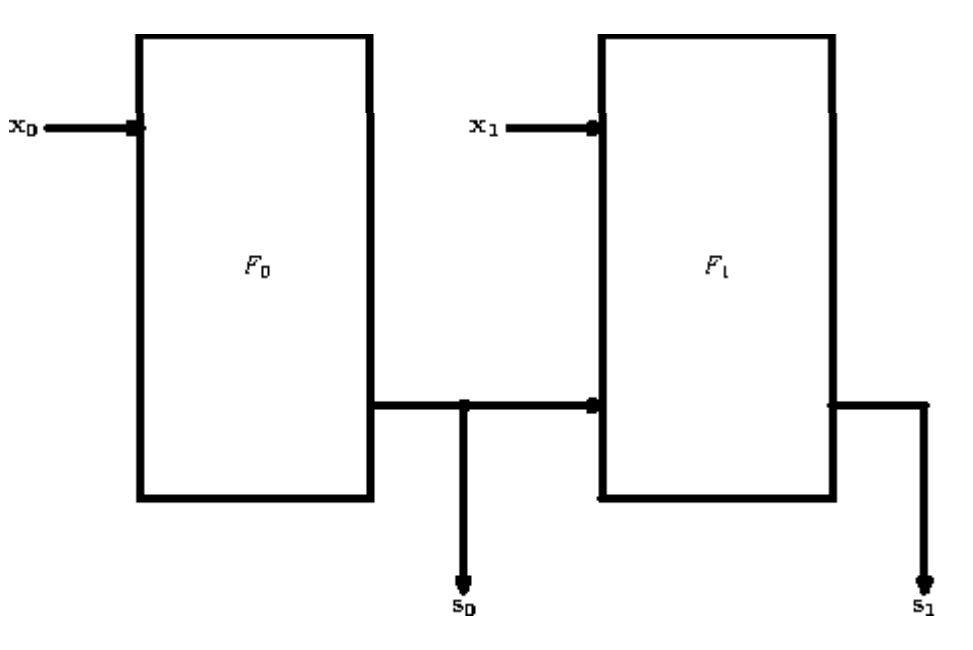
\includegraphics[width=0.55\textwidth]{Fig3.png}
\caption{Структура каскадной схемы.}
\label{fig:3}
\end{figure}

\begin{figure}[h!]
\centering
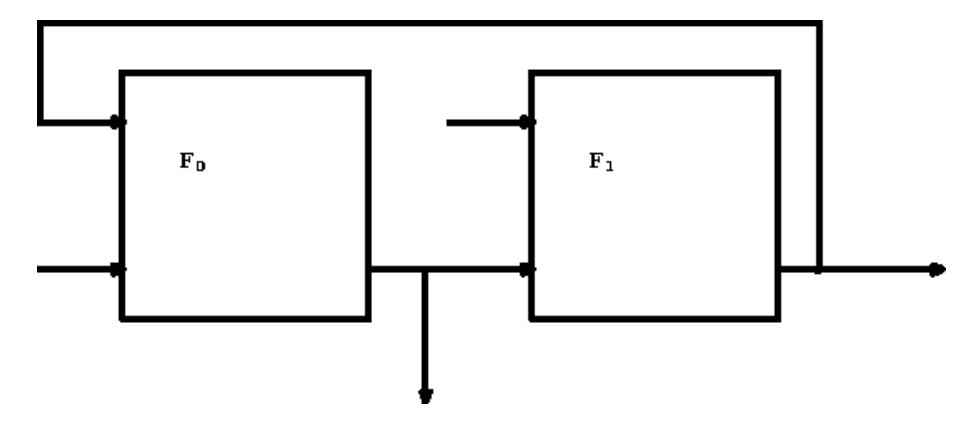
\includegraphics[width=0.55\textwidth]{Fig4.png}
\caption{Схема с глобальной обратной связью.}
\label{fig:4}
\end{figure}

\subsection{Матрица соединений}

Предположим, что обе схемы \(F_0\) и \(F_1\) заданы своими матрицами соединений \(\mathrm{Conn0}\) и \(\mathrm{Conn1}\). Чтобы построить матрицу \(\mathrm{Conn}\), относящуюся к возникшей схеме, нужно указать соединения между схемами \(F_0\) и \(F_1\). Мы можем сделать это с помощью двух списков \(\mathrm{FromF_0toF_1}\) и \(\mathrm{FromF_1toF_0}\). Каждый список содержит записи вида: индекс выхода и индекс свободного входа. Метод вычисления индекса свободного входа представлен в определении матрицы соединений. Продемонстрируем эти обозначения на примере схемы на рис.~2. Эту схему можно построить из двух схем на рис.~5 и рис.~6.

\begin{figure}[h!]
\centering
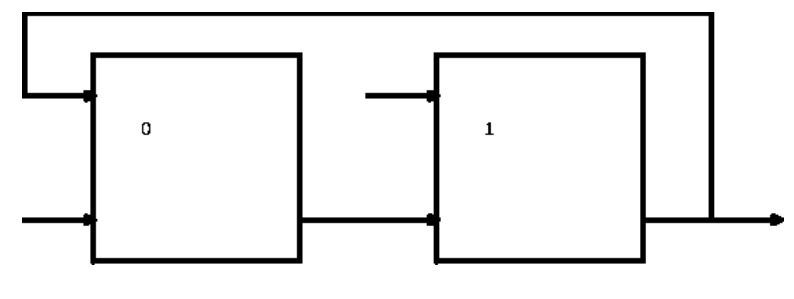
\includegraphics[width=0.45\textwidth]{Fig5.png}
\caption{Схема \(F_0\).}
\label{fig:5}
\end{figure}

\begin{figure}[h!]
\centering
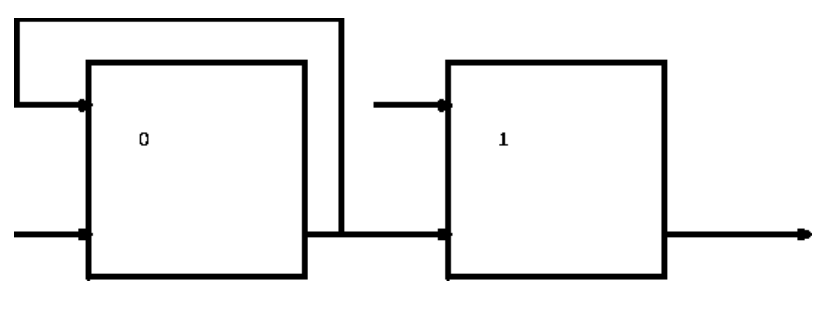
\includegraphics[width=0.45\textwidth]{Fig6.png}
\caption{Схема \(F_1\).}
\label{fig:6}
\end{figure}

Матрицы соединений имеют вид:

\[
\mathrm{Conn0} = 
\begin{pmatrix}
0 & 1 & 1 & 0\\
1 & 0 & 0 & 1
\end{pmatrix},
\qquad
\mathrm{Conn1} = 
\begin{pmatrix}
1 & 0 & 1 & 0\\
1 & 0 & 0 & 1
\end{pmatrix}.
\]

Списки, определяющие связи, имеют вид \(\mathrm{FromF_0toF_1} = [[1,0]]\) и \(\mathrm{FromF_1toF_0} = [[1,0]]\). Алгоритм вычисления матрицы соединений представлен в алгоритме 2.

\paragraph{Алгоритм 2. Вычисление матрицы соединений на основе матриц соединений \(F_0\) и \(F_1\)}
\begin{enumerate}
\item \(N_0, \mathrm{Col}_0 \leftarrow \mathrm{Conn0}\) \{размер матрицы, \(N_0\) --- число вентилей\}
\item \(N_1, \mathrm{Col}_1 \leftarrow \mathrm{Conn1}\)
\item \(L_{n0} \leftarrow \mathrm{FromF_0toF_1}\) \{длина списка\}
\item \(L_{n1} \leftarrow \mathrm{FromF_1toF_0}\)
\item \(N \leftarrow N_0 + N_1\) \{число вентилей\}
\item \(\mathrm{Col} \leftarrow \mathrm{Col}_0 + \mathrm{Col}_1 - L_{n0} - L_{n1}\)
\item \(\mathrm{Conn} \leftarrow\) нулевая матрица размера \(N \times \mathrm{Col}\)
\item \(\mathrm{Conn}[0:N_0, 0:N_0] \leftarrow \mathrm{Conn0}[:, 0:N_0]\)
\item \(\mathrm{Conn}[N_0:N, \mathrm{Col}_0:\mathrm{Col}_0 + N_1] \leftarrow \mathrm{Conn1}[:, 0:N_1]\)
\item \textbf{for} запись \textbf{in} \(\mathrm{FromF_0toF_1}\) \textbf{do}
\item \quad установить соединение, соответствующее записи
\item \quad удалить свободный вход из \(\mathrm{Conn0}\)
\item \textbf{end for}
\item \textbf{for} запись \textbf{in} \(\mathrm{FromF_1toF_0}\) \textbf{do}
\item \quad установить соединение, соответствующее записи
\item \quad удалить свободный вход из \(\mathrm{Conn1}\)
\item \textbf{end for}
\item добавить свободные входы в \(\mathrm{Conn}\)
\end{enumerate}

После генерации матрицы \(\mathrm{Conn}\) согласно алгоритму 2 появляется возможность объединять свободные входы. Для этого нужно переместить все объединяемые свободные входы в один столбец \(\mathrm{Conn}\), сохраняя позицию в столбце. Например, если в схеме на рис.~2 оба свободных входа объединены, то матрица соединений имеет вид

\begin{equation}
\mathrm{Conn} = 
\begin{pmatrix}
0 & 1 & 0 & 1 & 0\\
1 & 0 & 0 & 0 & 1\\
0 & 1 & 1 & 0 & 0\\
0 & 0 & 1 & 0 & 1
\end{pmatrix}. \label{eq:2}
\end{equation}

После построения матрицы соединений матрица переходов генерируется алгоритмом 1.

\subsection{Модульная схема как генератор}

Если устройство предназначено для генерации случайных значений, оно не должно иметь устойчивых состояний. Априори устройство, возможно, не сможет изменить своё состояние. Например, предположим, что выполняется уравнение

\begin{equation}
\begin{pmatrix}
1 \\
0
\end{pmatrix}
=
\begin{pmatrix}
0 & 1 & 1 \\
1 & 0 & 1
\end{pmatrix}
\odot_i
\begin{pmatrix}
1 \\
0 \\
1
\end{pmatrix}
\label{eq:3}
\end{equation}

для \(i = 0,1\). Это означает, что состояние \(\langle 1,0 \rangle\) устойчиво, если на свободный вход подана 1.

В [18] доказано необходимое и достаточное условие отсутствия устойчивых состояний у устройства. Чтобы сформулировать его, введём некоторые обозначения. Пусть \(\mathrm{Ident}\) --- единичная матрица, \(N\) --- число вентилей, \(\beta\) --- вектор, подаваемый на свободные входы. Устройство не имеет устойчивых состояний тогда и только тогда, когда

\begin{equation}
\rank(\mathrm{Ident} + \mathrm{Conn}[:,0:N])
<
\rank\bigl((\mathrm{Ident} + \mathrm{Conn}[0:N,0:N]) \mid \Delta\bigr), \label{eq:4}
\end{equation}

где \(\Delta = \mathrm{Conn}[:,N:]\beta^{\mathrm{T}}\) --- обычное матричное произведение над \(GF(2)\), а вертикальная черта обозначает добавление столбца к матрице. Очевидно, нулевое состояние всегда устойчиво, если \(\beta\) --- нулевой вектор. В дальнейшем мы исключаем эту ситуацию. Условие \eqref{eq:4} можно очень легко проверить в автоматическом режиме при проектировании схемы. В [14] доказано следующее утверждение.

\paragraph{Теорема.} Каскадная схема на рис.~3, где \(F_0\) --- инвертор, реализованный как сумматор с обратной связью, а другой вход установлен в 1, не имеет устойчивых состояний.

Например, схема на рис.~4 не имеет устойчивых состояний, когда оба блока эквивалентны блокам типа на рис.~6:

\begin{equation}
\mathrm{Conn} =
\begin{pmatrix}
1 & 0 & 0 & 1 & 0 & 0 \\
1 & 0 & 0 & 0 & 1 & 0 \\
0 & 1 & 1 & 0 & 0 & 0 \\
0 & 0 & 1 & 0 & 0 & 1
\end{pmatrix}. \label{eq:5}
\end{equation}

Следующим шагом в изучении свойств генератора является получение диаграммы переходов и поиск существования финального распределения для вектора \(\langle P_0(t),\allowbreak P_1(t),\allowbreak \dots,\allowbreak P_{K-1}(t) \rangle\) при \(t \to \infty\). Если единственное финальное распределение существует, то оно является нормированным собственным вектором матрицы переходов \(T_r\), относящимся к собственному значению \(N\). Возможно, что кратность собственного значения \(N\) больше 1. В этом случае для получения финального распределения требуется дополнительное рассмотрение.

\subsection{Реализация случайных генераторов для скрытой передачи информации}

В этом разделе мы представляем процедуру скрытой передачи данных по открытому каналу. Основная идея хорошо известна. Информация передаётся в виде сигнала, который выглядит как белый шум. Получатель анализирует сигнал с помощью известного алгоритма. Здесь мы представляем возможную реализацию этой идеи. Исследуем схему на рис.~7.

\begin{figure}[h!]
\centering
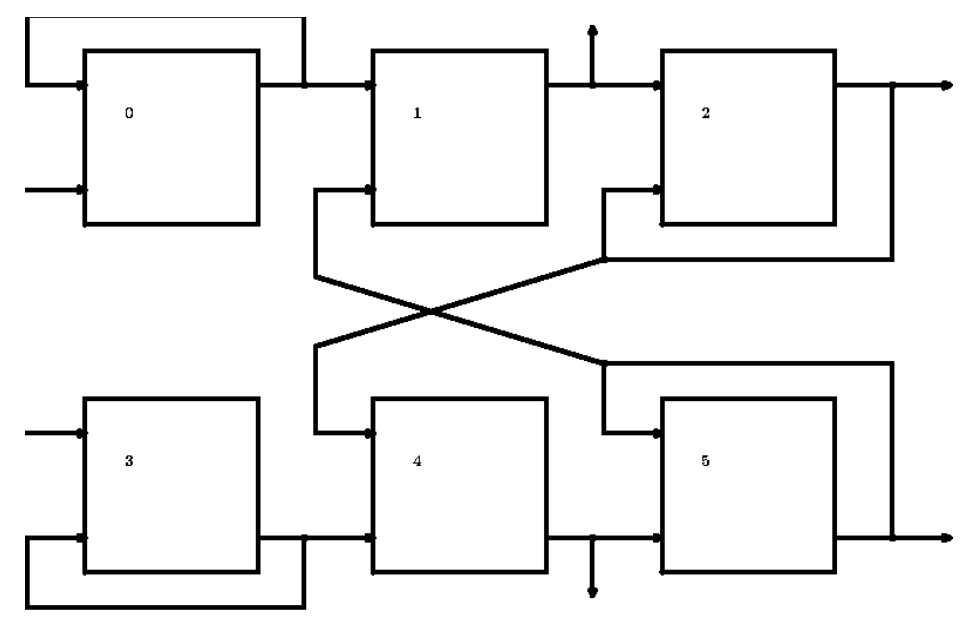
\includegraphics[width=0.7\textwidth]{Fig7.png}
\caption{Схема для реализации скрытой передачи данных.}
\label{fig:7}
\end{figure}

Это упрощённый вариант устройства. Можно расширить схемное решение на случай произвольного числа вентилей. Все утверждения, аналогичные сформулированным ниже, справедливы и для таких расширенных версий. Схема имеет два свободных входа, а выход схемы состоит из выходов вентилей 1, 2, 4, 5. Матрица соединений имеет вид

\[
\mathrm{Conn} =
\begin{pmatrix}
1 & 0 & 0 & 0 & 0 & 0 & 1 & 0 \\
1 & 0 & 0 & 0 & 0 & 1 & 0 & 0 \\
0 & 1 & 1 & 0 & 0 & 0 & 0 & 0 \\
0 & 0 & 0 & 1 & 0 & 0 & 0 & 1 \\
0 & 0 & 1 & 1 & 0 & 0 & 0 & 0 \\
0 & 0 & 0 & 0 & 1 & 1 & 0 & 0
\end{pmatrix}.
\]

Допустимыми сигналами на свободных входах являются \((1,0)\), \((0,1)\) и \((1,1)\). Согласно теореме, схема не имеет устойчивых состояний, пока на свободные входы подаётся один из допустимых сигналов.

Рассмотрим ситуацию, когда подаётся входной вектор \((1,0)\). В этом случае сигнал на выходе вентиля 3 будет постоянным. Таким образом, диаграмма переходов генератора содержит по крайней мере две связные компоненты. Прямое вычисление спектра матрицы \(T_{r10}\) показывает, что кратность собственного значения 6 равна 2. Следовательно, мы имеем ровно две связные компоненты на диаграмме переходов. С другой стороны, \(T_{r11}\) имеет единственный собственный вектор, относящийся к собственному значению 6. Все компоненты этого вектора положительны. Это означает, что диаграмма переходов имеет единственную связную компоненту и каждое состояние достижимо из любого другого состояния.

Идея скрытой передачи данных состоит в следующем. Сопоставим \((1,0)\) с 1, \((0,1)\) с 0, а \((1,1)\) с пробелом между двумя символами в исходном файле. Обозначим эти три сигнала как управляющие сигналы генератора.

Предполагается, что интервал между двумя тактовыми импульсами в синхронном регистре (рис.~1) достаточно велик, чтобы марковский процесс перешёл в состояния, близкие к финальному распределению. Сравним вероятности различных состояний в финальном распределении при подаче управляющих сигналов. В нашем случае выходной вектор имеет длину 4.

Прежде всего сравним вероятности при подаче векторов \((1,0)\) и \((0,1)\). Из-за симметрии схемы выходные вероятности для \((0,0,0,0)\), \((0,1,1,0)\), \((1,0,0,1)\) и \((1,1,1,1)\) будут одинаковыми. Различия изображены на рис.~8.

\begin{figure}[h!]
\centering
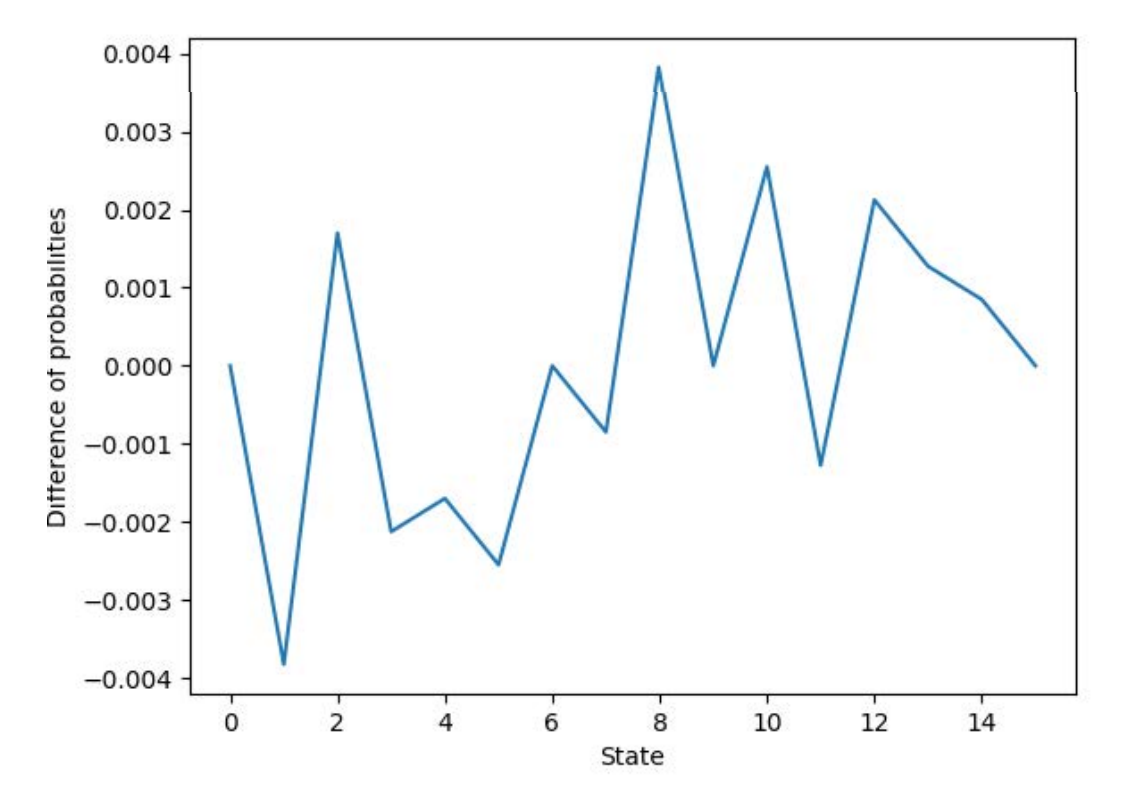
\includegraphics[width=0.7\textwidth]{Fig8.png}
\caption{Разности вероятностей различных состояний для управляющих сигналов \((0,1)\) и \((1,0)\).}
\label{fig:8}
\end{figure}

Из рис.~8 следует, что наиболее значимые различия достигаются для векторов \(\mathbf{1} = (0,0,0,1)\) и \(\mathbf{8} = (1,0,0,0)\), поэтому, используя эти два сигнала в качестве маркеров, можно различать управляющие сигналы и биты информации.

Чтобы выделить пробел между двумя битами, нужно сравнить вероятности при подаче на свободные входы \((0,1)\), \((1,0)\) и \((1,1)\). Эти различия представлены на рис.~9.

\begin{figure}[h!]
\centering
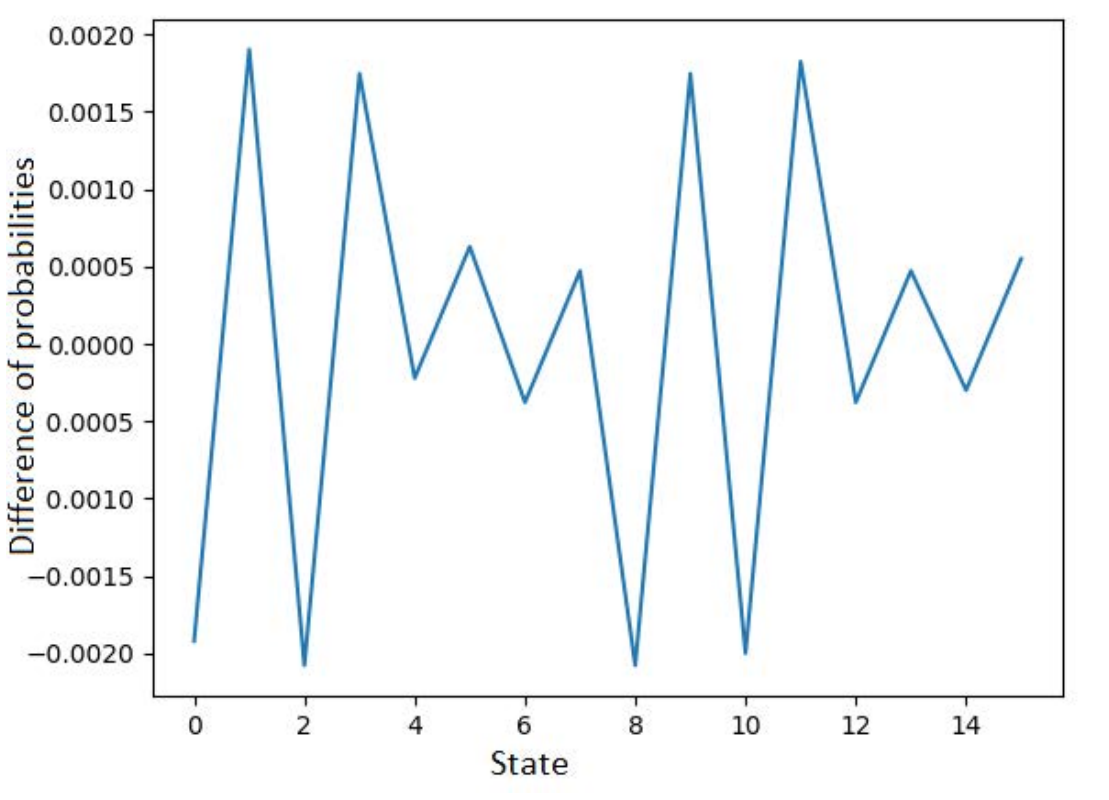
\includegraphics[width=0.7\textwidth]{Fig9.png}
\caption{Разности вероятностей при подаче \((1,0)\) и \((1,1)\) для реализации скрытой передачи данных.}
\label{fig:9}
\end{figure}

Из рис.~8 и рис.~9 следует, что разнообразие сигналов можно использовать для обнаружения управляющего сигнала. Число тактов (длина случайной последовательности), используемое для передачи одного бита с заданной надёжностью, является стандартной задачей, известной как проверка гипотез [19,20].

\section{Заключение}

Разработано новое семейство истинно случайных генераторов чисел в виде каскадных (модульных) схем. Теоретические исследования, а также эксперименты показывают пригодность генератора для скрытой передачи данных.

\begin{thebibliography}{20}

\bibitem{1} R.~Langmann, O.~Makarov, L.~Meyer, and S.~Nesterenko, ``The WOAS project: web-oriented automation system,'' \textit{9th Int. Conf. on Remote Engineering and Virtual Instrumentation}, pp.~1--2, 2012.

\bibitem{2} A.~Faul, N.~Jazdi, and M.~Weyrich, ``Approach to interconnect existing industrial automation systems with the Industrial Internet,'' \textit{IEEE 21st Int. Conf. on Emerging Technologies and Factory Automation}, pp.~1--4, 2016.

\bibitem{3} Z.~Bi, L.~Hu, and C.~Wang, ``Internet of Things for Enterprise Systems of Modern Manufacturing,'' \textit{IEEE Transactions on Industrial Informatics}, vol.~10, is.~2, pp.~1537--1546, 2014.

\bibitem{4} A.~Sadeghi, C.~Wachsmann, and M.~Waidner, ``Security and privacy challenges in industrial Internet of Things,'' \textit{52nd ACM/EDAC/IEEE Design Automation Conf.}, pp.~1--6, 2015.

\bibitem{5} W.~Granzer, F.~Praus, and W.~Kastner, ``Security in building automation systems,'' \textit{IEEE Transactions on Industrial Electronics}, vol.~57, is.~11, pp.~3622--3630, 2010.

\bibitem{6} T.~Muller, A.~Walz, M.~Kiefer, and H.~Doran, ``Challenges and Prospects of Communication Security in Real-Time Ethernet Automation Systems,'' \textit{14th IEEE Int. Workshop on Factory Communication Systems}, pp.~1--9, 2018.

\bibitem{7} J.~Zhang, T.~Duong, A.~Marshall, and R.~Woods, ``Key Generation From Wireless Channels: A Review,'' \textit{IEEE Access}, vol.~4, pp.~614--626, 2016.

\bibitem{8} M.~Ma, D.~He, N.~Kumar, and K.~Choo, ``Certificateless Searchable Public Key Encryption Scheme for Industrial Internet of Things,'' \textit{IEEE Transactions on Industrial Informatics}, vol.~14, is.~2, pp.~759--767, 2018.

\bibitem{9} D.~Holcomb, W.~Burleson, and K.~Fu, ``Power-Up SRAM State as an Identifying Fingerprint and Source of True Random Numbers,'' \textit{IEEE Transactions on Computers}, vol.~58, is.~9, pp.~1198--1210, 2009.

\bibitem{10} M.~Ni, A.~Parihar, A.~Raychowdhury, and S.~Datta, ``Stochastic insulator-to-metal phase transition-based true random number generator,'' \textit{IEEE Electron. Device Letters}, vol.~39, is.~1, pp.~139--142, 2018.

\bibitem{11} A.~Johnson, R.~Chakraborty, and D.~Mukhopaday, ``An improved DCM-based tunable true random number generator for Xilinx FPGA,'' \textit{IEEE Transactions on Circuits and Systems II: Express Briefs}, vol.~64, is.~4, pp.~452--456, 2017.

\bibitem{12} E.~Kim, M.~Lee, and J.~Kim, ``8.2 8Mb/s 28Mb/mJ robust true-random-number generator in 65nm CMOS based on differential ring oscillator with feedback resistors,'' \textit{IEEE Int. Solid-State Circuits Conf.}, pp.~144--145, 2017.

\bibitem{13} R.~Latypov and E.~Stolov, ``Asynchronous linear combinational circuits as a base for programmable logic device. Binary and ternary cases,'' \textit{IFAC-PapersOnLine}, vol.~49, is.~25, pp.~378--383, 2016.

\bibitem{14} R.~Latypov and E.~Stolov, ``Theory of ternary jitter-based true random number generators composed of identical gates,'' \textit{Scientists Notes of Kazan University. Series of Physics and Mathematics}, vol.~159, is.~2, pp.~246--262, 2017.

\bibitem{15} F.~Gantmacher, \textit{Applications of the Theory of Matrices}. NY: Dover Publications, 2005.

\bibitem{16} A.~Howard, \textit{Elementary Linear Algebra (Applications Version)}. Wiley International, 2005.

\bibitem{17} R.~Latypov and E.~Stolov, ``A new family of controlled ternary true random number generators,'' \textit{IEEE East-West Design and Test Symposium}, pp.~1--6, 2018.

\bibitem{18} V.~Kuznetsov, V.~Pesoshin, and E.~Stolov, ``Markov model of a digital stochastic generator,'' \textit{Automation and Remote Control}, vol.~69, is.~9, pp.~1504--1509, 2008.

\bibitem{19} H.~Kramer, \textit{Mathematical method of statistics}. Princeton: Princeton University Press, 1999.

\bibitem{20} A.~Borovkov, \textit{Mathematical Statistics}. Boca Raton: CRC Press.

\end{thebibliography}

\end{document}